\documentclass[MTech]{iitmdiss}

\usepackage{times}
\usepackage{setspace}
\usepackage{amsmath,amsthm,amssymb,amsfonts}
\usepackage{verbatim}
\usepackage{floatrow}
\usepackage{fullpage}
\usepackage{listings}
%\usepackage{txfonts,pxfonts,amsfonts}
\usepackage[usenames,dvipsnames]{xcolor}


\usepackage{xcolor}
\usepackage{caption}
\usepackage{subfig}
\usepackage{graphicx}

\usepackage[square]{natbib}
\usepackage[colorlinks=true,linkcolor=black]{hyperref}
%\usepackage{hyperref} % hyperlinks for references.
\usepackage[all]{hypcap}
\usepackage{complexity}
\usepackage[named]{algo}
%\usepackage{algpseudocode}
\newtheorem{thm}{Theorem}
\newtheorem{problem}{Problem}
\newtheorem{corr}{Corollary}
\newtheorem{lma}{Lemma}
\newtheorem{case}{Case}
\newtheorem{rmrk}{Remark}
\newtheorem{prp}{Proposition}
\newtheorem{dfn}{Definition}
\newtheorem{qn}{Question}
\newtheorem{att}{Attempt}
\newtheorem{ex}{Example}
\newtheorem{flaw}{Flaw in Attempt}
\usepackage{bm}
\usepackage{xcolor}
\usepackage{float}
\xdefinecolor{gray}{rgb}{0.4,0.4,0.4}
\xdefinecolor{blue}{RGB}{58,95,205}% R's royalblue3; #3A5FCD

% Strut macros for skipping spaces above and below text in tables. 
\def\abovestrut#1{\rule[0in]{0in}{#1}\ignorespaces}
\def\belowstrut#1{\rule[-#1]{0in}{#1}\ignorespaces}

\def\abovespace{\abovestrut{0.20in }}
\def\aroundspace{\abovestrut{0.20in}\belowstrut{0.10in}}
\def\belowspace{\belowstrut{0.10in}}
%%%%%%%%%%%%%%%%%%%%%%%%%

\lstset
{
	numbers=left,
    breaklines=true,
    postbreak=\raisebox{0ex}[0ex][0ex]{\ensuremath{\color{red}\hookrightarrow\space}}
}

\def\thesistitle{}
\def\thesisauthor{D Akshay Rangasai}


\begin{document}
\bibliographystyle{iitm}
%%%%%%%%%%%%%%%%%%%%%%%%%%%%%%%%%%%%%%%%%%%%%%%%%%%%%%%%%%%%%%%%%%%%%% 
% Title page

\title{\thesistitle}

\author{\thesisauthor}

\date{May 2015}
\department{Mechanical Engineering}

%\nocite{*}
\begin{singlespace}
\maketitle 
\end{singlespace} 

%%%%%%%%%%%%%%%%%%%%%%%%%%%%%%%%%%%%%%%%%%%%%%%%%%%%%%%%%%%%%%%%%%%%%%
% Certificate
\certificate

\vspace*{0.5in}

\noindent This is to certify that the thesis entitled {\bf {\thesistitle}}, 
submitted by {\bf {\thesisauthor}}, to the Indian Institute of Technology, 
Madras, for the award of the degree of {\bf Master of Technology}, 
is a bona fide record of the research work carried out by him under my
supervision. The contents of this thesis, in full or in parts, have not been
submitted to any other Institute or University for the award of any degree or
diploma.

\vspace*{1.4in}
\hspace*{-0.25in}
\begin{minipage}{0.5\textwidth}
\begin{singlespace}
\noindent {\bf Krishnan Balasubramanian} \\
\noindent Research Guide \\ 
\noindent Professor \\
\noindent Dept. of Mechanical Engineering\\
\noindent IIT-Madras, 600 036 \\
\end{singlespace}
\end{minipage}
\begin{minipage}{0.5\textwidth}
\begin{singlespace}
\noindent {\bf L Vijayaraghavan} \\
\noindent Research Co-Guide \\ 
\noindent Professor \\
\noindent Dept. of Mechanical Engineering\\
\noindent IIT-Madras, 600 036 \\
\end{singlespace}
\end{minipage}
\vspace*{0.20in}
\noindent Place: Chennai\\ 
Date:

%%%%%%%%%%%%%%%%%%%%%%%%%%%%%%%%%%%%%%%%%%%%%%%%%%%%%%%%%%%%%%%%%%%%%%
\acknowledgements
I want to thank myself for this completely pointless endeavour and my parents for paining me constantly about this. This is in the end, quite depressing.
%%%%%%%%%%%%%%%%%%%%%%%%%%%%%%%%%%%%%%%%%%%%%%%%%%%%%%%%%%%%%%%%%%%%%%
% Abstract

\abstract
Most materials have two regimes of operation when it comes to the relationship between stress and strain of the material, namely linear and non-linear. while phenomenon and material characterization in the linear regime of operation is pretty well understood, the non-linear regime is not as well understood. This is an intriguing part of the problem as materials that undergo plastic deformation and fatigue loading operate under this non-linear regime, and characterization of these properties help in various manufacturing processes.

This study aims to statistically model and extract relevant parameters to measure non-linearity and its effects on a material by the use of ultrasonic waves, which provide a high strain rate, but very low strain, which is ideal to test the material without changing any of its properties at the current state. We first characterize parameters through harmonics generation and then proceed to non-linear wave mixing, a technique which gives us spatial specificity in our measurements. 

The forward model was first built by creating a Finite Difference Time Domain (FDTD) solution to a set of differential equations that represent two dimensional non-linear wave propagation in an isotropic solid medium in a euclidean coordinate system. Wave mixing was simulated using a transverse and a longitudinal wave mixing in collinear path, with a phased array simulated as the transducer. Sensitivity analysis was performed for this solution and this formed the basis of our inverse model that helped predict material parameters.

The inverse model for the forward model was first built using linear regression and the results were compared with a statistical learning technique. We used Gaussian Process modelling to model the predictive model, which we further used to build the inverse model. To evaluate the model, noise was added to the measurements at various Signal to Noise Ratio (SNR) and the error percentage was measured. This model proved to be sufficient for the inverse model. From this, we could effectively estimate model parameters from wave mixing measurements.

The thesis further explores the directions this work could take along with the applications of the said techniques. By expanding on the dimensionality and complexity of the problem, we can effectively use this technique to monitor as well as improve manufacturing processes. 
\pagebreak

%%%%%%%%%%%%%%%%%%%%%%%%%%%%%%%%%%%%%%%%%%%%%%%%%%%%%%%%%%%%%%%%%
% Table of contents etc.

\begin{singlespace}
\tableofcontents
\thispagestyle{empty}

\listoftables
\addcontentsline{toc}{chapter}{LIST OF TABLES}
\listoffigures
\addcontentsline{toc}{chapter}{LIST OF FIGURES}
\end{singlespace}

\pagebreak


%The main text will follow from this point so set the page numbering
%to arabic from here on.
\pagenumbering{arabic}
%%%%%%%%%%%%%%%%%%%%%%%%%%%%%%%%%%%%%%%%%%%%%%%%%%
% Introduction.
%\input{misc.tex}
%\input{questions.tex}
\chapter{Introduction}

The subject of the present work deals with the propagation, non-linear mixing effects of high-frequency shear and longitudinal waves which help us characterize material properties. This section is a brief introduction containing the background, outline and applications of the presented work.

\section{Background}
The stress-strain curve for most ductile materials starts in a linear relationship and moves into a non-linear relationship with a few invariants that define the said relationship. Determining these constants is of great use to characterize the material and predict its behaviour under various conditions and also optimize processes with respect to these constants. While the physical relationship between the linear constants and their estimation has been studied to a great extent, the non-linear constants are more difficult to estimate. Our work aims to estimate these non-linear constants through statistical estimation techniques.

\subsection{The stress-strain curve}
\begin{center}
\begin{figure}[ht]
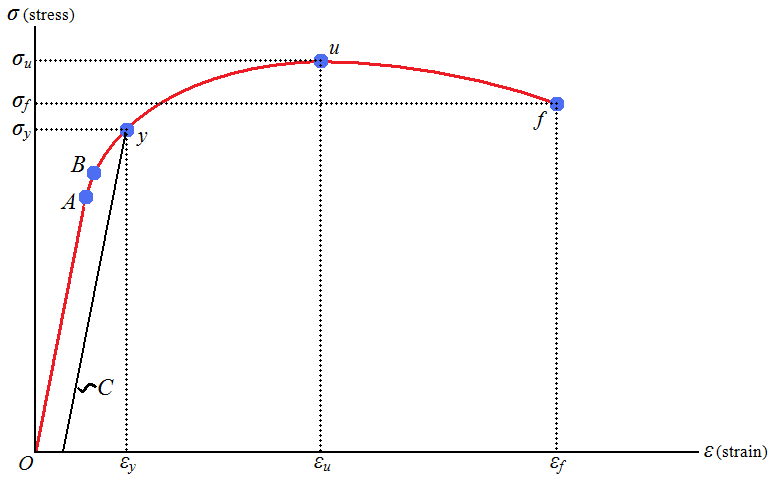
\includegraphics[scale=0.45]{images/chapter_1/stressstrain.png}
\caption{The Stress Strain Curve for a Typical Material}
\end{figure}
\end{center}
The significant points from fig 1.1.1 are as follows:
\begin{enumerate}
\item A - Proportional Limit
\item B - Elastic Limit
\item y - Yield Point
\item u - Ultimate Tensile Strength
\item f - Fracture point
\end{enumerate}
\subsection{Non-Destructive Testing}
There are multiple methods of figuring out the elastic constants of a material, most significant of them being destructive methods, where the material is stressed to its Ultimate Tensile Strength and then, a curve is fit to get the second order constants of the material. This results in the material specimen being destroyed and deemed useless. This method is good for laboratory conditions, but not in a real-world scenario.

To account for this, we employ a method of Non-Destructive testing using ultrasonics. Ultrasonic waves have the characteristic of extremely high strain rates, but the magnitude of strain itself is minimal, and the changes to material properties are thus negligible. These high strain rates result in interesting phenomenon occurring, which in turn helps us estimate parameters of the material, without any physical damage to the specimen.

\subsection{Wave Propagation and Mixing}
One of the main concepts that are used in this study are that of wave propagation in solid media and mixing of waves in linear and non-linear zones. To solve the differential equations involved, we use FDTD simulations. We employed multiple solvers to evaluate the equations and multiple approaches to solve the problem. This will be discussed in detail in upcoming chapters.

\subsection{Statistical Inversion and Learning}
The forward model is inverted by using purely statistical techniques. We employ various techniques from Support Vector Machines (SVM), Gaussian Mixture Models (GMMs), and Gaussian Processes. The mathematics and results will be discussed in detail in the coming chapters.
\section{Outline of the Report}
This report is organized into 6 chapters.
\begin{enumerate}

\item The current chapter gives a basic introduction to the project and explains very briefly what we hope to achieve and techniques we've employed with a little bit of background information.

\item Chapter 2 deals with Literature Review and what we worked on and the subsequent results of the same with reasons as to what method we finally adopted and why with a discussion about the same.

\item Chapter 3 describes the construction of the FDTD model for the forward problem and the collinear wave mixing approach that is taken by us and describes the problem and solution in detail.

\item Chapter 4 explores the sensitivity analysis of our constructed forward model with respect to various parameters of interest and and exploratory analysis of the inverse model.

\item Chapter 5 validates the inverse model and also describes the pitfalls of the model. We make the model more real world friendly and check its performance.

\item Chapter 6 summarizes our work and has a section on how this project can be pursued along with suggestions for experimental validation.
\end{enumerate}
\section{Applications of present work}
The present work has wide range of uses from aircraft industry to the shipping industry. A manufacturing specific application of this current technique will be in the estimation of material parameters in forming process and cold working processes where materials undergo plastic deformation. 

This technique will help us understand material deformation better and give us a physical insight into what the constants mean and at the same time help improve existing processes and diagnose issues in current processes.  

\chapter{Literature Review}
\section{Introduction}
to first understand the problem at hand and look at how to proceed, a literature survey was undertaken by us. We scoured through multiple scientific journals and used them as markers for our work. Due to the relative similarity of this problem to that faced in photonics/optics, many papers from an Electrical/Quantum Mechanical background were found. A few papers that developed theory rigorously were also looked at. Below, we shall list out the most important papers in our survey and also explain what each paper contributed to this project. Post that, we describe the approach we plan to take to tackle the problem at hand.


\section{Paper Review}

The first paper is from 1971, from an old soviet journal \cite{zarem} This paper develops the theory from first principles and attempts to solve it using relatively older numerical techniques. This paper clearly explains non-linear phenomena in solid. This paper formed the base of our future work, and our first simulation solver was based on the ideas given in this paper. The paper, besides the rigorous mathematical treatment of the subject at hand, also delves into phonon interaction in materials in brief.

With this background, we derive that there are only a few modes of mixing that is accepted in a material, and these criteria converge whichever approach you take to treat the subject. With a basic phonon treatment of the subject matter, the nuances of wave mixing are also discussed. This is very important and acts as the base on which the rest of the project is built.

This paper was implemented initially, and the results were quite accurate, but this didn't quite serve the purpose of what we set out to do and thus we switched our starting point.

%Put table of Wave Mixing and possible modes and shit. Diagrams also

\begin{figure}
\begin{center}
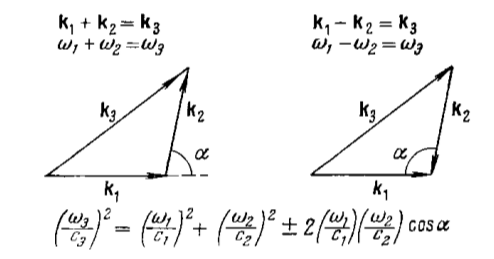
\includegraphics[scale=0.5]
{images/chapter_2/directions_noncollinear.png}
\caption{Direction of resultant wave\cite{zarem}}
\end{center}
\end{figure}

\begin{figure}
\begin{center}
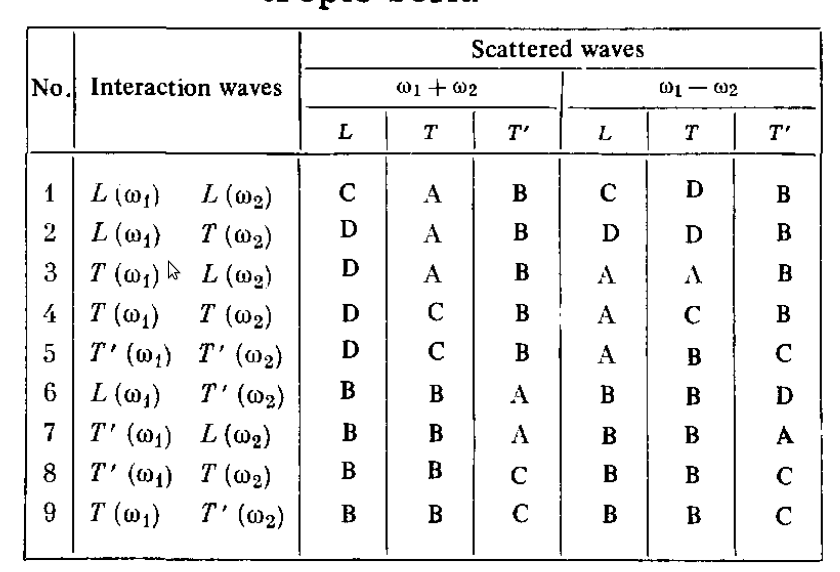
\includegraphics[scale=0.5]
{images/chapter_2/interaction.png}
\caption{Forbidden Modes of Wave Mixing \cite{zarem}}
\end{center}
\end{figure}

The second paper that was pursued post this was a paper on three phonon interaction and a quantum(light) analogue applied to solid material. This paper further expounded on acceptable modes of mixing and also the direction and wave-characteristics of the resulting wave. However, the approach taken by the authors in the paper seemed far too advanced for our purposes and thus this paper was used for experimental setup than the starting point for our work.


The third paper of great significance was that by Liu \cite{Liu}. This paper had a very classical treatment of the governing equation and its solution in a 2 Dimensional collinear environment. The paper was not too advanced and proved useful as our starting point in the simulations. 

The differential equations derived are in two dimensions and could be solved easily. an FDTD method approach was taken over any other approach due to the flexibility of FDTD methods. This paper formed the basis of the forward model and sensitivity analysis. Based on this and a few other readings, we decided to take this approach to tackle the problem.

\begin{figure}
\begin{center}
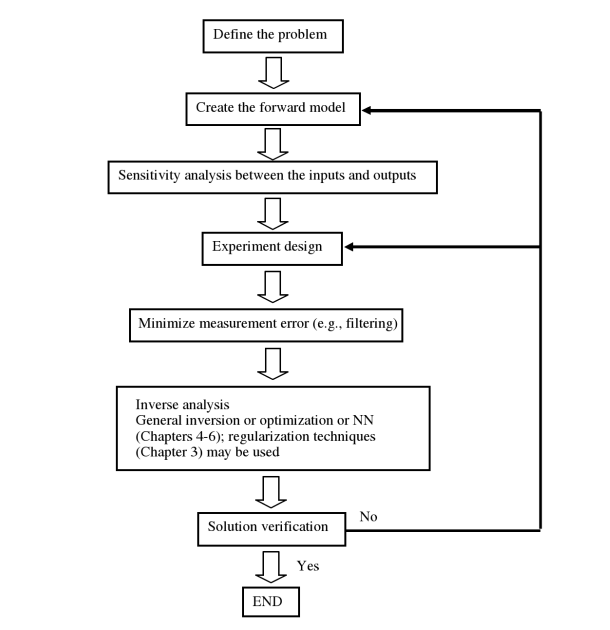
\includegraphics[scale=1]
{images/chapter_2/mthodology_generic.png}
\caption{Generic Methodology of this Project}
\end{center}
\end{figure}

For the inverse model, most of the literature was read from Bishop \cite{bishop} and a few other PhD thesis. This marks the end of literature survey and implementation details of the project
\chapter{Description Of Simulations}
This chapter presents the description of the simulations used for the current research. The objective of the simulation is to estimate the amplitude and frequency of the resultant generated wave post mixing. This is primarily due to the non-linear behaviour of the material in the mixing zone. The following are the steps followed to achieve this objective.

% Fancy Graphic Explaining What I will be doing%

\section{2D FDTD Simulation in Cartesian Coordinates}
Finite Difference Time Domain (FDTD) method is widely used to solve wave propagation problems. In the present work the FDTD algorithm is implemented in 2D Orthogonal Cartesian Coordinates. \cite{yee}
\section{Governing Equations}
The primary governing equations for the 2D FDTD simulator are the non-linear wave propagation equations in the material. Let $u(y,t)$, $v(y,t)$ describe the motion of wave propagation for a longitudinal and transverse wave in a solid.  The equations can be derived as such from the standard equation of motion in a solid material.


\begin{equation}
\frac{\partial \sigma_{xy}}{\partial y} = \rho \frac{\partial^2 u}{\partial t^2}
\end{equation}

\begin{equation}
\sigma_{xy} = \sigma{yx} = \frac{\partial u}{\partial y}(\mu + m\frac{\partial v}{\partial y})
\end{equation}

\begin{equation}
\frac{\partial \sigma_{yy}}{\partial y} = \rho \frac{\partial^2 v}{\partial t^2}
\end{equation}

In terms of the Lame constants $\lambda$ and $\mu$, and the third order elastic constants l, m, and n (the Murnaghan coefficients), the stress components can be related to the displacement gradients through + \cite{derive_step_1}

\begin{equation}
\sigma_{yy} = (\lambda + 2 \mu)\frac{\partial v}{\partial y} + (l + 2m)\frac{\partial v}{\partial y}^2 + \frac{m}{2}\frac{\partial u}{\partial y}^2
\end{equation}

Substituting the previous two relations to the standard wave equation, we get

\begin{equation}
\frac{ \partial^2 u }{\partial t^2} - c_t^2 \frac{\partial^2 u}{\partial y^2} = \beta_t c_t^2 \frac{\partial}{\partial y}(\frac{\partial u}{\partial y} \frac{\partial v}{\partial y})
\end{equation}

\begin{equation}
\frac{ \partial^2 v }{\partial t^2} - c_l^2 \frac{\partial^2 v}{\partial y^2} = \beta_l c_l^2 \frac{\partial v}{\partial y}\frac{\partial^2 v}{\partial y^2} + \beta_t c_t^2 \frac{\partial u}{\partial y}\frac{\partial^2 u}{\partial y^2}
\end{equation}
Where, $c_L = \sqrt{(\lambda + 2\mu)\\\rho}$, $c_T = \sqrt{\mu \\\rho}$
\begin{equation}
\beta_L = 3 + \frac{2(l + m)}{\lambda + 2\mu}
\end{equation}
\begin{equation}
\beta_T = \frac{\lambda + 2\mu}{\mu} + \frac{m}{\mu}
\end{equation}

\subsection{Discretization of the wave-equation}
This wave equation, can be discretized as a FDTD grid, which using the staggered method of FDTD solver along with the central differencing technique results in a equation similar to this:
\begin{equation}
\begin{aligned}
\frac{u^{n+1}_{k} - 2*u^n_k + u^{n-1}_k}{\Delta t^2} = \\
 & c_T^2\frac{u^n_{k+1} - 2 u^n_k + u^n_{k-1}}{\Delta y^2} \\
+ &  \beta_T c_T^2(\frac{u^n_{k+1} - 2 u^n_k + u^n_{k-1}}{\Delta y^2}\frac{v^n{k+1} 
- v^n_{k-1}}{2\Delta y} \\
+ & \frac{v^n_{k+1} - 2 v^n_k + v^n_{k-1}}{\Delta y^2}\frac{u^n{k+1} - u^n_{k-1}}{2\Delta y})
\end{aligned}
\end{equation}
\begin{equation}
\begin{aligned}
u^{n+1}_{k} = \\
& 2*u^n_k - u^{n-1}_k +  \Delta t^2 c_T^2(\frac{u^n_{k+1} - 2 u^n_k + u^n_{k-1}}{\Delta y^2} \\
+ & \beta_T (\frac{u^n{k+1} - u^n_{k-1}}{2\Delta y}\frac{u^n_{k+1} - 2 u^n_k + u^n_{k-1}}{\Delta y^2} +\frac{v^n_{k+1} - 2 v^n_k + v^n_{k-1}}{\Delta y^2}\frac{u^n{k+1} - u^n_{k-1}}{2\Delta y}))
\end{aligned}
\end{equation}
\begin{figure}
\begin{center}
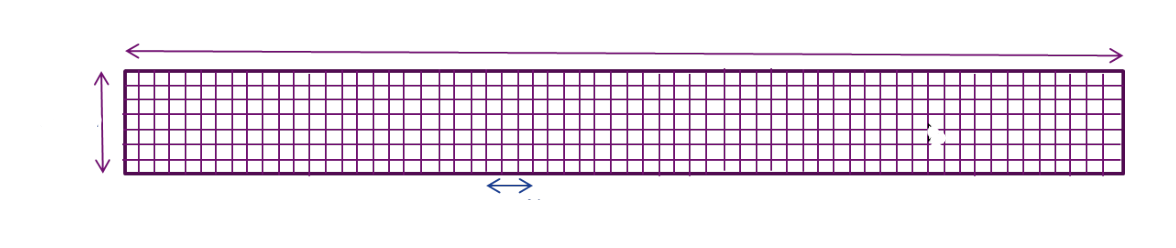
\includegraphics[scale=0.4]{images/chapter_3/schematic_GE.png}
\caption{Schematic of the solid material as an FDTD grid}
\end{center}
\end{figure}
\begin{figure}
\begin{center}
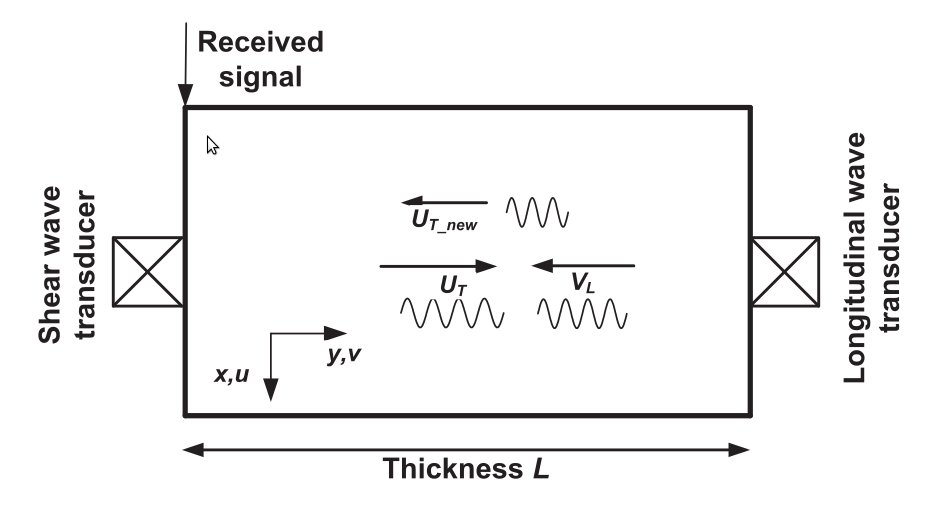
\includegraphics[scale=0.4]{images/chapter_3/schematic_liu.jpg}
\caption{Schematic of the setup the FDTD simulation is mimicking}
\end{center}
\end{figure}
\subsection{Numerical Considerations}
\subsubsection{Stability Criteria}
A finite difference scheme is stable if the errors made at one time step of the calculation do not cause the errors to increase as the computations are continued. A neutrally stable scheme is one in which errors remain constant as the computations are carried forward. If the errors decay and eventually damp out, the numerical scheme is said to be stable. If, on the contrary, the errors grow with time the numerical scheme is said to be unstable. The stability of numerical schemes can be investigated by performing von Neumann stability analysis. For time-dependent problems, stability guarantees that the numerical method produces a bounded solution whenever the solution of the exact differential equation is bounded. Stability, in general, can be difficult to investigate, especially when the equation under consideration is non-linear. \\
In the FDTD for sound waves, the main stability criteria is the \textbf{Courant} condition. This constraint ensures that the errors in the numerical simulation get damped out to give a fairly accurate  estimate of the actual solution.
\begin{equation}
\Delta t \leq \frac{1}{C} \frac{1}{\sqrt{\frac{1}{(\Delta x)^2}+\frac{1}{(\Delta y)^2}}}
\end{equation}
\begin{equation}
\Delta x = \Delta y,
\Delta t \leq \frac{1}{C} \frac{1}{\sqrt{2}}
\end{equation}
Where $C$ is the velocity of the wave and $\Delta x$ is the spatial discretizarion in metre and $\Delta t$ is the temporal discretization.
\subsubsection{Boundary Conditions}
The simulation needs a few boundary conditions to be set up, such that there is a solution to the equation that is solved. In this case, we assume the propagation of the wave as equal to the propagation of a wave through any standard wave guide. Since, we are assuming a metal-to-air interface, we have modeled this as a completely reflecting wave guide with no absorption. For other interfaces or absorption in the wave-guide, we could look at a Perfectly Matched Layers (PML) at the boundaries for complete absorption.

The wave guide is modeled as a free waveguide on all ends and the movement is not restricted anywhere. For such a scenario, in the case of plane wave propagation in solids, it is the particle displacement at the boundary which is free, and nothing else. In case the ends are not free to move, the particle displacements at the boundary are trivial. For both these cases, we see reflections, but there is a phase inversion that happens in the latter case. This is not of great importance in this context, but helps validate simulations.

The conditions for the same implemented in the code is as follows.
\begin{equation}
u^n_{-1} = u^n_{-2}
\end{equation}
\begin{equation}
v^n_{-1} = v^n_{-2}
\end{equation}
Where $-1, -2$ denote the grid points from the boundaries, with $-1$ being the last grid point.
\subsubsection{Initial condition}
Another important component of the boundary layer is basically the initial conditions of the simulation itself. This determines the initial state of the system and the excitement that is given to the system and determines the outcome of the simulation. 

For this FDTD simulation, we need to excite the system with one transverse and one longitudinal wave on either end. As the system we have currently taken is collinear, the only criteria is the excitation, and nothing else. The initial wave forms must also be smooth\cite{smoothness} to prevent numerical dispersion and dissipation errors in the simulations \cite{errors} \cite{errors_2}

\subsection{Mesh and Sampling Sampling}
To further get a more accurate solution, we have to choose a suitable size of mesh for which the solution is acceptable and at the same time not too time consuming. The solution must be approximately right, without too much noise in the data. The solution is also sampled at a rate which is extremely high to prevent aliasing of the data. We sample at a rate that is proportional to the meshing, a criteria we get from the courant condition.

\section{Simulation}
\subsection{Sources}
There are two main sources in the simulations, one is a longitudinal wave with a specific frequency and another is a transverse wave coming in from the opposite direction. These are limited in time, and thus are pulses of waves. The pulses are raised cosine pulses with a pulse width of 10. 
\begin{figure}
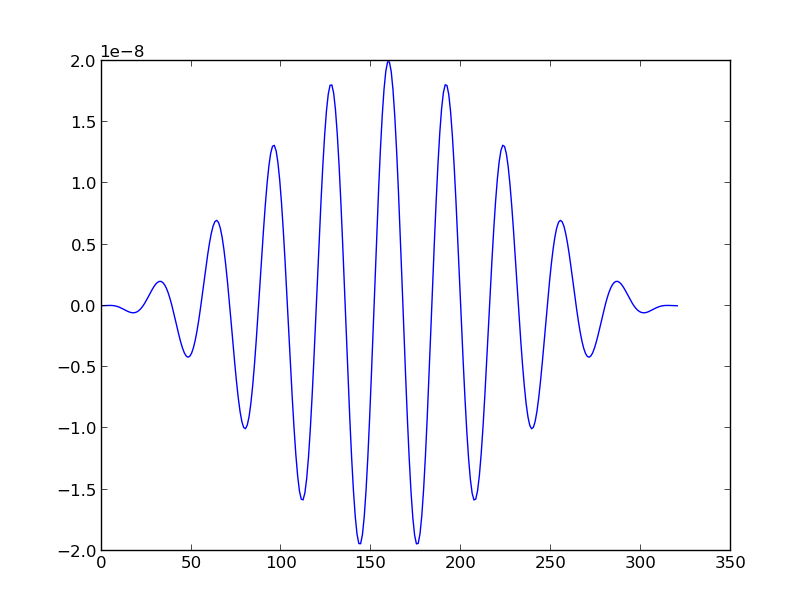
\includegraphics[scale=0.5]{images/chapter_3/wave_1.png}
\caption{Longitudinal Pulse Excited at Source}
\end{figure}
\begin{figure}
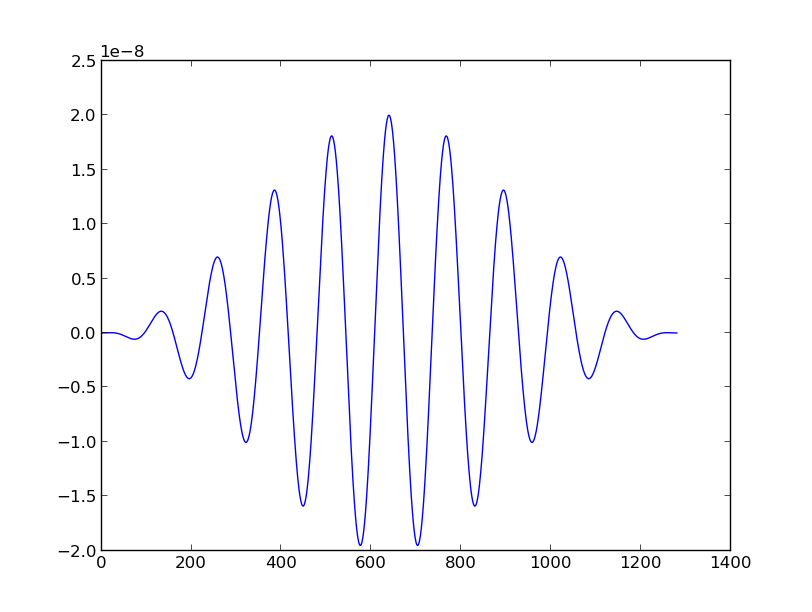
\includegraphics[scale=0.5]{images/chapter_3/wave_2.png}
\caption{Transverse Pulse Excited at Source}
\end{figure}
\subsection{Simulation Parameters}
\begin{table}[ht]
\caption{General Numerical Properties of Simulation}
\begin{tabular}{|c|c|}
\hline
\textbf{Property} & \textbf{Value} \\ \hline
$\Delta t$ & $3.125 \times 10^{-09}$s \\ \hline
$\Delta x$ & $3.94 \times 10^{-05}$m \\ \hline
Sampling Frequency & $3.2 \times 10^{8}$Hz \\ \hline
\end{tabular}
\end{table}
\begin{table}[ht]
\caption{Pulse Properties}
\begin{tabular}{|c|c|c|}
\hline
\textbf{Property} & \textbf{Longitudinal} & \textbf{Transverse} \\ \hline
Number of pulses & 10 & 10 \\ \hline
Pulse Frequency(MHz) & 10MHz & 2.5MHz \\ \hline
Pulse Amplitude (m) & $2 \times 10^{-8}$m & $2 \times 10^{-8}$m \\ \hline
Pulse Duration (s) & $10^{-6}$s & $4 \times 10^{-6}$s \\ \hline
Pulse Velocity $ms^{-1}$ & $6299.5ms^{-1}$ & $3100ms^{-1}$\\ \hline 
\end{tabular}
\end{table}
\section{Simulation Results}
\subsection{Snapshots of Simulation}
\begin{figure}[ht]
\centering
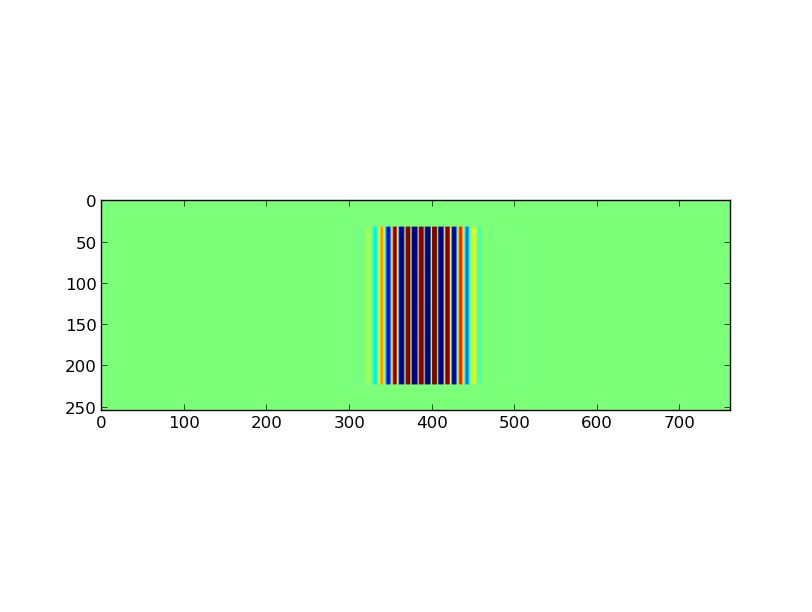
\includegraphics[scale=0.5]{images/chapter_3/simulation_picture_long.png}
\caption{Snapshot of the Longitudinal Wave}
\end{figure}

\begin{figure}[ht]
\centering
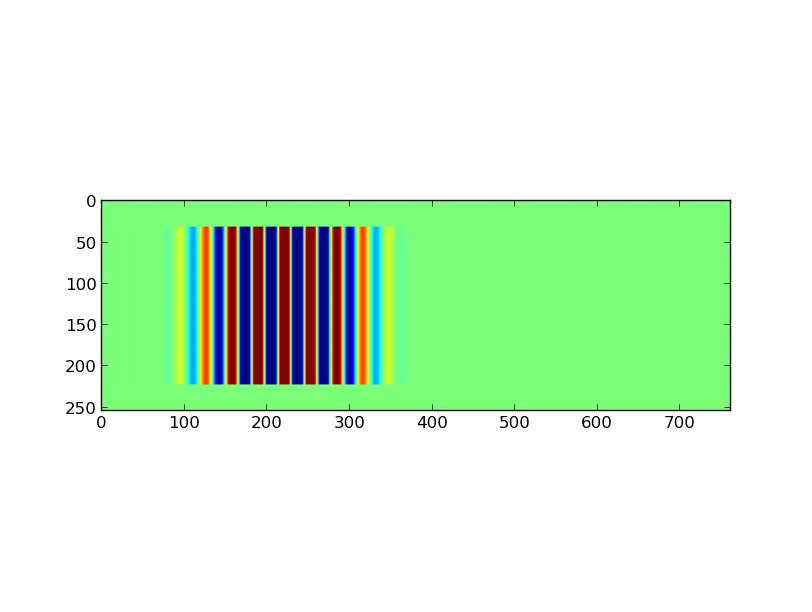
\includegraphics[scale=0.6]{images/chapter_3/simulation_picture_transverse.png}
\caption{Snapshot of the Transverse Wave}
\end{figure}

\begin{figure}[!ht]
\centering
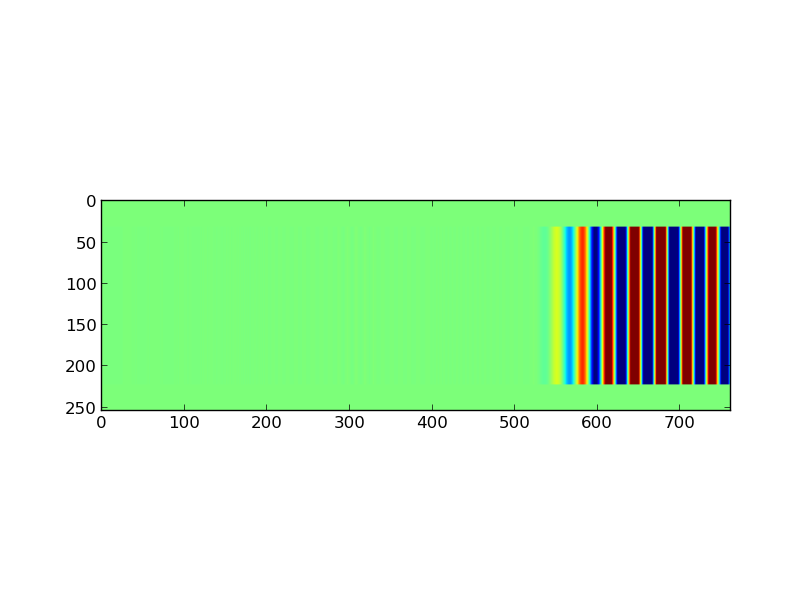
\includegraphics[scale=0.6]{images/chapter_3/wave_trans.png}
\caption{Snapshot of the Transverse Wave}

\end{figure}

\subsection{Validation of Simulation}
The solution from the simulation was obtained from an Amplitude Scan at both the sources. The wave forms and the fourier transforms of the waves after the A-scans were consistent with what is expected from an FDTD simulation. There was minimal dispersion or dissiparion error and thus the simulation parameters were satisfactory. To check if the FDTD simulation is accurate enough to be used for more complex cases with the same solver and engine, we compared the results of our FDTD simulation with the one by Liu Et. al \cite{Liu} which solved this case by the use of an ODE solver. 

From the comparisons of the two solutions, we compared the scale of amplitude as well as the frequency of the generated wave. Due to our input being markedly different from that of the reference paper, the deviations in wave shape are acceptable. All the other criteria match with that of the reference paper. The comparisons and Validation plots are given below.


\begin{figure}[ht]
\begin{center}
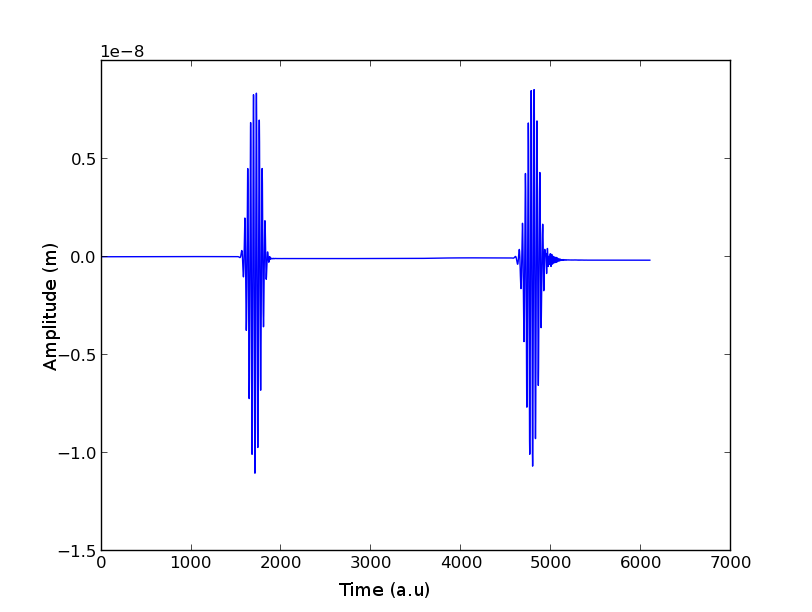
\includegraphics[scale=0.7]{images/chapter_3/final_longitudinal.png}
\caption{A-scan of the longitudinal wave}
\end{center}
\end{figure}

\begin{figure}[ht]
\begin{center}
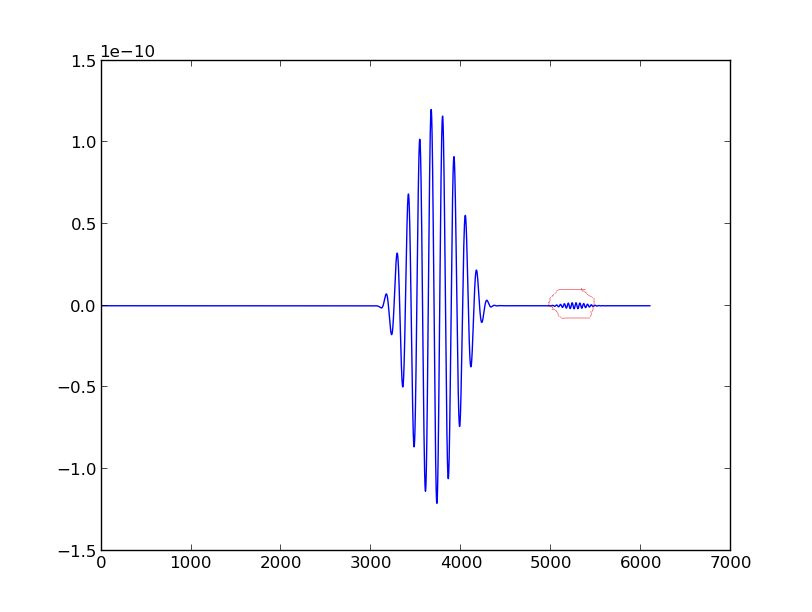
\includegraphics[scale=0.5]{images/chapter_3/final_transverse.png}
\caption{A-scan of the transverse wave}
\end{center}
\end{figure}

\begin{figure}[ht]
\begin{center}
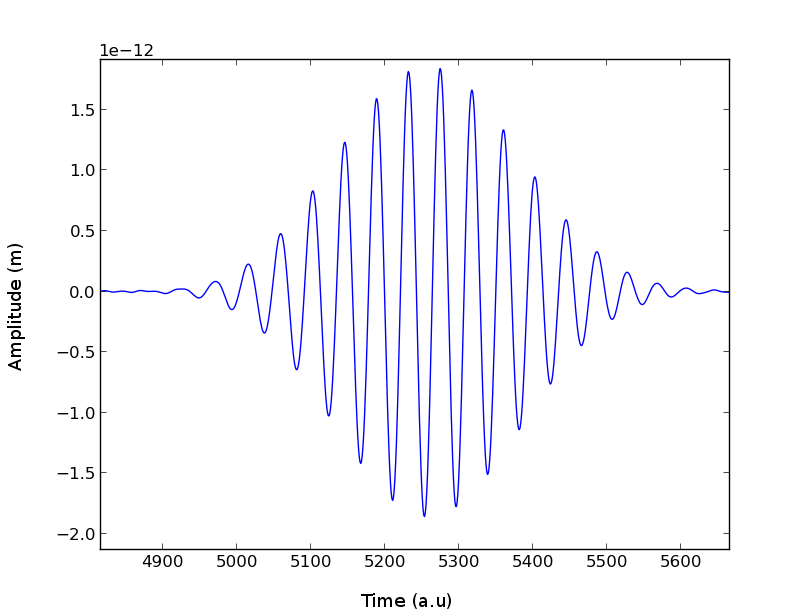
\includegraphics[scale=0.5]{images/chapter_3/final_transervse_zoom.png}
\caption{Zoomed A-scan of transverse wave}
\end{center}
\end{figure}


\begin{figure}
\begin{center}
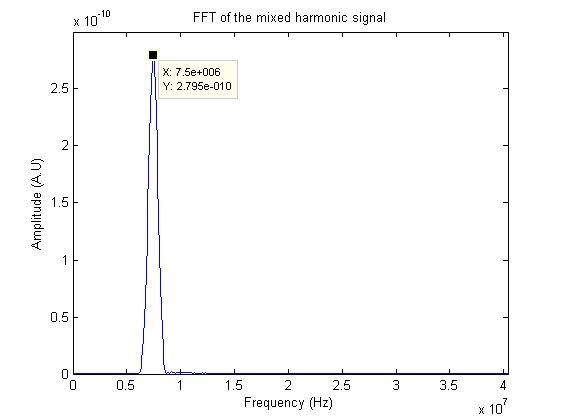
\includegraphics[scale=0.5]{images/chapter_3/finaLfft_zzom.jpg}
\caption{Fourier Transform of the New Wave Generated}
\end{center}
\end{figure}

\begin{figure}
\begin{center}
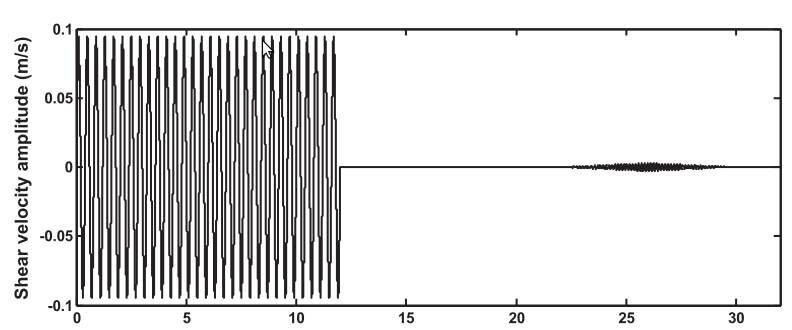
\includegraphics[scale=0.5]{images/chapter_3/validation.png}
\caption{Simulation Results From DE solver\cite{Liu}}
\end{center}
\end{figure}

\begin{figure}
\begin{center}
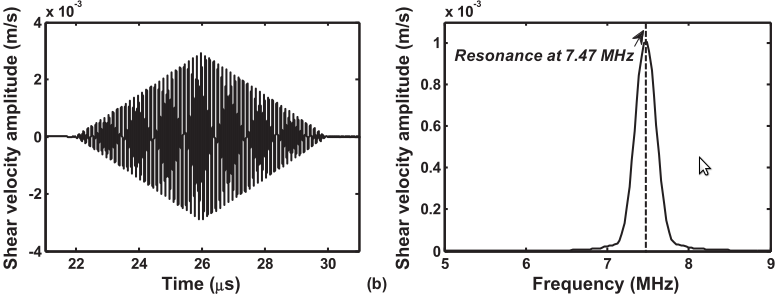
\includegraphics[scale=0.5]{images/chapter_3/validation_2.png}
\caption{Zoomed solution and Fourier Transform of the solution from DE solver \cite{Liu}}
\end{center}
\end{figure}
\chapter{Sensitivity Analysis}
\section{Introduction}
A mathematical model is defined by a series of equations, input variables and parameters aimed at characterizing some process under investigation. Increasingly, such models are highly complex, and as a result their input/output relationships may be poorly understood. In such cases, the model can be viewed as a black box, i.e. the output is an opaque function of its inputs.

Quite often, some or all of the model inputs are subject to sources of uncertainty, including errors of measurement, absence of information and poor or partial understanding of the driving forces and mechanisms. This uncertainty imposes a limit on our confidence in the response or output of the model. Further, models may have to cope with the natural intrinsic variability of the system (aleatory), such as the occurrence of stochastic events.

Good modeling practice requires that the modeler provides an evaluation of the confidence in the model. This requires, first, a quantification of the uncertainty in any model results (uncertainty analysis); and second, an evaluation of how much each input is contributing to the output uncertainty. Sensitivity analysis addresses the second of these issues (although uncertainty analysis is usually a necessary precursor), performing the role of ordering by importance the strength and relevance of the inputs in determining the variation in the output.

In models involving many input variables, sensitivity analysis is an essential ingredient of model building and quality assurance. 

\section{Objectives of Sensitivity Analysis}
The objective of sensitivity analysis is typically dictated by a number of problem constraints or settings.


\textbf{Correlated inputs}

Sometimes inputs can be strongly correlated. If done correctly, sensitivity analysis helps us understand the correlations and extract important features from the model.

\textbf{Model interactions }

Interactions occur when the perturbation of two or more inputs simultaneously causes variation in the output greater than that of varying each of the inputs alone. Sensitivity analysis helps capture those variations and understand the process better. This is an invaluable tool to capture such information.

Another useful feature of sensitivity analysis is that it helps capture non-linearities in a model. For a black-box model with an input and an output, sensitivity analysis helps determine non-linearities.



\subsection{Caveats while performing sensitivity analysis}


\textbf{Computational expense}

Sensitivity analysis is almost always performed by running the model a (possibly large) number of times, i.e. a sampling-based approach. This can be a significant problem when, A single run of the model takes a significant amount of time (minutes, hours or longer). This is not unusual with very complex models.

The model has a large number of uncertain inputs. Sensitivity analysis is essentially the exploration of the multidimensional input space, which grows exponentially in size with the number of inputs. See the curse of dimensionality.

Computational expense is a problem in many practical sensitivity analyses. Some methods of reducing computational expense include the use of emulators (for large models), and screening methods (for reducing the dimensionality of the problem). Another method is to use an event-based sensitivity analysis method for variable selection for time-constrained applications.[6] This is an input variable selection method that assembles together information about the trace of the changes in system inputs and outputs using sensitivity analysis to produce an input/output trigger/event matrix that is designed to map the relationships between input data as causes that trigger events and the output data that describes the actual events. The cause-effect relationship between the causes of state change i.e. input variables and the effect system output parameters determines which set of inputs have a genuine impact on a given output. The method has a clear advantage over analytical and computational IVS method since it tries to understand and interpret system state change in the shortest possible time with minimum computational overhead.

\textbf{Correlated inputs}

Most common sensitivity analysis methods assume independence between model inputs, but sometimes inputs can be strongly correlated. This is still an immature field of research and definitive methods have yet to be established.

\textbf{Non-linearity}

Some sensitivity analysis approaches, such as those based on linear regression, can inaccurately measure sensitivity when the model response is nonlinear with respect to its inputs. In such cases, variance-based measures are more appropriate.

\textbf{Model interactions }

Interactions occur when the perturbation of two or more inputs simultaneously causes variation in the output greater than that of varying each of the inputs alone. Such interactions are present in any model that is non-additive, but will be neglected by methods such as scatterplots and one-at-a-time perturbations.[8] The effect of interactions can be measured by the total-order sensitivity index.

\textbf{Multiple outputs}

Virtually all sensitivity analysis methods consider a single univariate model output, yet many models output a large number of possibly spatially or time-dependent data. Note that this does not preclude the possibility of performing different sensitivity analyses for each output of interest. However, for models in which the outputs are correlated, the sensitivity measures can be hard to interpret.


\section{Methodology}

\subsection{Generic Procedure}
Most procedures adhere to the following steps for a sensitivity analysis:

\begin{enumerate}

\item Quantify the uncertainty in each input (e.g. ranges, probability distributions)

\item Identify the model output to be analysed 

\item Run the model a number of times using some design of experiments

\item Using the resulting model outputs, calculate the sensitivity measures of interest.

\end{enumerate}

\subsection{Approach for forward model}
The approach to our sensitivity analysis was two-fold. Our parameters of interest are the higher order elastic coefficients l,m. We perturb this value from 90\% of their initial value to 110\% of that value. By increasing at a step of 1\%, this results in 441 simulations, which within the constraints of time and computation power seemed excessive. Before doing this analysis, we took a One at a Time approach, to check if there were dependencies between l,m in our output. 

Using this one at a time approach, values of l and m were varied by keeping one of the other constant. This resulted in about 42 simulations with a few duplicates. Many more simulations were run with $\beta_t$ as one of the parameters, but since the dependency of  $\beta_t$ to l,m is known, it was not an independent variable and thus these data points were discarded. The results were then plotted and a covariance matrix was built, to check for dependencies. Based on the plots and covariance matrix, these simulations were deemed enough to proceed with the inverse model.

\begin{figure}
\begin{center}
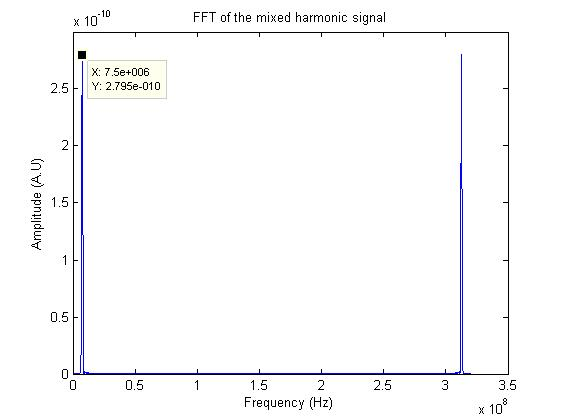
\includegraphics[scale=0.5]{images/chapter_4/finaLfft_nozzom.jpg}
\caption{FFT of generated wave}
\end{center}
\end{figure}

\begin{figure}
\begin{center}
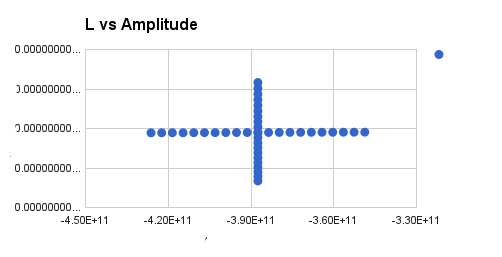
\includegraphics[scale=0.7]{images/chapter_4/lvsamp.png}
\caption{effect of l on the amplitude of generated wave}
\end{center}
\end{figure}

\begin{figure}
\begin{center}
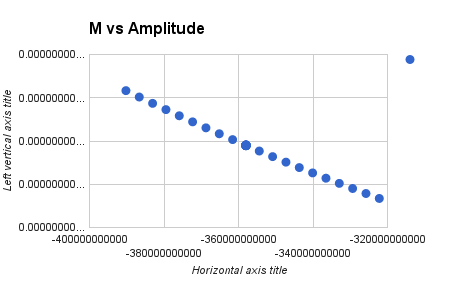
\includegraphics[scale=0.7]{images/chapter_4/mvsamp.png}
\caption{effect of m on the amplitude of generated wave}
\end{center}
\end{figure}
\section{Results and Discussion}
From the plots of amplitude of resultant wave with respect to the perturbation of constants, it is clear that amplitude changes only with changes in the value of m, and is agnostic to the value of l. One of the reasons for this could be because of the problem under consideration itself. We are working with collinear mixing where one degree of freedom is lost while waves are mixing. Another reason is the mixing of transverse and longitudinal waves result in a transverse wave which is affected only by this constant in a 2D situation. For a non-collinear approach, this would change significantly. Due to multiple interactions happening in the material.

All the resulting waves had a similar peak frequency, and thus frequency of the resultant wave wasn't used further for modelling the inverse.
\chapter{Inverse Model}
\section{Introduction}
In the classical problem, we deal with a set of input variables resulting in an output y. This method of getting an output using known inputs is known as the forward model. What if the inputs weren't measurable, but are of significance and the output is the only measurable quantity. This problem is known as the inverse model, where for a relationship that goes from $A \longrightarrow B$, we figure out the elements of $A$ from the elements of $B$. 

Before we invert the model itself, we run our techniques on the forward model to determine its accuracy.  
\section{Fitting the forward model}
\subsection{Linear Regression}
For the forward model, we have the values of l,m and the amplitude of the wave that is generated. Using the given parameters of l,m we must determine the relationship between l,m and amplitude. The first step that we have taken is the linear regression. The mathematical formulation of linear regression is shown below.
$$\textbf{X} = [l m]$$
$$b = [A]$$
\begin{equation}
A\textbf{X} = \textbf{b}
\end{equation}
For a non-square matrix X
\begin{equation}
A = (XX^T)^{-1}X^Tb
\end{equation}

The linear regression of the forward model 
\subsection{The Gaussian Process}
\section{Statistical Techniques}
\subsection{Noisy data}
The data we have worked with till now has been data without any noise added to it. To validate the model, it is necessary to have a dataset that is contaminated with a few errors in sampling. Thus, to emulate an actual transducer's signal, we add noise to the data at Various SNRs. The results at various SNRs are compared to test the accuracy of the inverse model. Since we measure the amplitude of the resultant wave, the noise is added to the peak-to-peak amplitude value of the wave. 
\subsection{Adding Noise}
The Signal to Noise ratio for a signal can be defined as 

\begin{equation}
SNR = \frac{P_{signal}}{P_{noise}}
\end{equation}

\begin{equation}
SNR = \frac{\sigma^2_{signal}}{\sigma^2_{noise}}
\end{equation}

\begin{equation}
SNR = \frac{A^2_{signal}}{A^2_{noise}}
\end{equation}

To add noise to our amplitude signal, we calculate the power of the peak-to-peak amplitude signals, calculate the power and then add Gaussian white noise at a specific variance to match the desired Signal to Noise Ratio. In this case, we have worked with a signal to noise ratio from 2 to 20.
\subsection{The Gaussian Process}
Gaussian Processes for Machine Learning (GPML) is a generic supervised learning method primarily designed to solve regression problems.The gaussian process is a non-parametric method that works with hyperparameters. It is also a probabilistic method for regression.

The advantages of Gaussian Processes for Machine Learning are:
\begin{enumerate}
        \item The prediction interpolates the observations (at least for regular correlation models).
        \item The prediction is probabilistic (Gaussian) so that one can compute empirical confidence intervals and exceedance probabilities that might be used to refit (online fitting, adaptive fitting) the prediction in some region of interest.
        \item Versatile: different linear regression models and correlation models can be specified. Common models are provided, but it is also possible to specify custom models provided they are stationary.
\end{enumerate}
The disadvantages of Gaussian Processes for Machine Learning include:
\begin{enumerate}


        \item It is not sparse. It uses the whole samples/features information to perform the prediction.
        \item It loses efficiency in high dimensional spaces – namely when the number of features exceeds a few dozens. It might indeed give poor performance and it loses computational efficiency.
        \item Classification is only a post-processing, meaning that one first need to solve a regression problem by providing the complete scalar float precision output y of the experiment one attempt to model.

\end{enumerate}

Due to the nature of the Gaussian Process, it can be used to solve global optimization problems. From the given advantages and disadvantages of GPML, it fits perfectly for solving our inverse problem. A brief mathematical background is given for the Gaussian Process. Interested readers are requested to refer to \cite{gp} \cite{gp_tut} for a more rigorous treatment of this subject.

\subsection{Background of Gaussian Process}
The Gaussian Process instead of parametrizing the input output relationships of variables, instead assumes a prior over a distribution of functions. This helps eliminate the parametrization and associated pitfalls. Gaussian Process Treats each function as a sample from a multivariate Gaussian Distribution. Like a kernel method, it projects the finite dataset into an infinite dimensional space. To put it mathematically. Instead of parameterizing $y(\textbf{X},\textbf{w})$, we place a prior of $P(y(\textbf{x}))$. For the given data $D = {\textbf{X},\textbf{y}}$
\begin{equation}
p(\textbf{f}|\textbf{X}) = N(0,\textbf{K})
\end{equation}    
\begin{equation}
K(x,x') = E[f(x)f(x')]
\end{equation}
Now, for a GP regression, we can write $y$ as
\begin{equation}
y = f + \epsilon
\end{equation}
\begin{equation}
\epsilon = GWN(0,\sigma_e)
\end{equation}

For a test and train marginal likelihood,

\begin{equation}
p(y,y_t) = N(0, K_{N+T}) + \sigma^2_e \textbf{I}
\end{equation}

\begin{equation}
p(y_T | y) = N(\mu_T, \Sigma_T)
\end{equation}

The solutions to this formulation are beyond the scope of this dissertation and the reader is requested to consult the references mentioned above. This problem now becomes an optimization problem to minimize log likelihood. This gives us our solution.
\section{Discussion and Results}
\chapter{Summary and Future Work}
\section{Conclusion}
The estimation of higher order coefficients from amplitude data of collinear wave mixing is  a problem for which an inversion exists and thus, is solvable. During the course of the work undertaken, the forward problem proved to be more challenging than the inverse problem, to solve. This is simply because of the techniques employed for inversion. The inverse model and its results have shown less than an 8\% error in prediction, and thus is accurate within limits of acceptability.

The techniques used in the solution of this problem are taken from computer science and applied to this specific problem. The results have been quite encouraging, and this must be looked into further. The work done can act as the basis of much more advanced studies, and this will be explored further below. 

\section{Future Work}
The work described in this project can be extended further by using this as a strong foundation. This forms the framework for future work, which is exciting and has many real world applications. The specific case we have solved here, is one of the many cases of a generic problem. Added to that fact that it is constrained to the 2-Dimensional space currently, there is huge potential to build on this work.

\subsection{Theoretical}
Upgrading this from the 2D space to the 3D space is something that can be worked on. While this problem is non-trivial, it could prove to be challenging due to the sheer computational volume involved. With a 3D implementation, the possibilities of this simulation are endless.\cite{noncollinear} \cite{phd_thesis}

Multiple variations of this problem can be worked on, from going from an L-T wave mixing to a generic wave mixing scheme. The solver can be updated to solve for any sort of wave excitation. This will result in a much greater variety of solutions and possibilities in the future. With different wave mixing, other parameters can also be extracted from a material.

Finally, a non-collinear scheme can be developed for a similar use case. A non-collinear scheme is not only more directional but also localized in its solutions. This helps us analyze material and estimate parameters with extremely high accuracy. The trade off for such convenience is highly correlated variables which makes the inversion more involved.

Working in a similar vein, a manufacturing process can be simulated, for example, forming and the effects of the process on these constants can be estimated using a wave mixing technique. This could help optimise process parameters to get much better results and greater efficiency.

\subsection{Experimental}

Model validation can be pursued experimentally with a sample of a highly strained piece of material. While there is literature which has explored this path, the inversion from said data isn't something that has been carried out by them.

The technique can further be applied to specimens that undergo intense stress in manufacturing processes to understand said processes better. At multiple sages of forming, specimen can be evaluated to determine the constants values and this can be used to model the process better.

Non-collinear techniques can be experimented with. These techniques are more specific and local and grant the experimenter the freedom to set up his apparatus comfortably. For non-regular shapes, non-collinear wave mixing approach works better than a collinear one as it is more directional.

The references given on this page will direct the user to the potential and areas of work that can be focused on in the future.
%%%%%%%%%%%%%%%%%%%%%%%%%%%%%%%%%%%%%%%%%%%%%%%%%%%%%%%%%%%%
% Appendices.
\appendix
\chapter{Appendix}
\input{appendix.tex}
\section{Solver Code}
\lstinputlisting[language=Python]{../solver.py}
\pagebreak
\section{Problem Formulation Code}
\lstinputlisting[language=Python]{../formulation.py}
\pagebreak
\section{Material Data Setting Code and Constants}
\lstinputlisting[language=Python]{../data.py}
\lstinputlisting[language=Python]{../constants.py}
\pagebreak
\section{Code for Automating Simulations}
\lstinputlisting[language=Python]{../framework.py}
\pagebreak
\section{Code to Analyse Sensitivity}
\lstinputlisting[language=Python]{../sensitivity_analysis.py}
\pagebreak
\section{Inverse Model Code}
\lstinputlisting[language=Python]{../GMM_regression.py}
\pagebreak
\section{Defaults Code}
\lstinputlisting[language=Python]{../defaults.py}
% Bibliography.
\pagebreak
\chapter{Material Properties Used in Simulations}
%\begin{singlespace}
%  \begin{small}
%  	\bibliographystyle{plain}
%	\bibliography{bibliography}
%  \end{small}
%\end{singlespace}
\chapter{Closed Form Solution}
\begin{thebibliography}{9}
\input{bibliography.bib}
\end{thebibliography}
%%%%%%%%%%%%%%%%%%%%%%%%%%%%%%%%%%%%%%%%%%%%%%%%%%%%%%%%%%%%

\end{document}
